\documentclass[10pt]{beamer}
\usetheme[
%%% option passed to the outer theme
%    progressstyle=fixedCircCnt,   % fixedCircCnt, movingCircCnt (moving is deault)
  ]{Feather}
  
% If you want to change the colors of the various elements in the theme, edit and uncomment the following lines

% Change the bar colors:
%\setbeamercolor{Feather}{fg=red!20,bg=red}

% Change the color of the structural elements:
%\setbeamercolor{structure}{fg=red}

% Change the frame title text color:
%\setbeamercolor{frametitle}{fg=blue}

% Change the normal text color background:
%\setbeamercolor{normal text}{fg=black,bg=gray!10}

%-------------------------------------------------------
% INCLUDE PACKAGES
%-------------------------------------------------------

\usepackage[utf8]{inputenc}
\usepackage[english]{babel}
\usepackage[T1]{fontenc}
\usepackage{helvet}

%-------------------------------------------------------
% DEFFINING AND REDEFINING COMMANDS
%-------------------------------------------------------

% colored hyperlinks
\newcommand{\chref}[2]{
  \href{#1}{{\usebeamercolor[bg]{Feather}#2}}
}

%-------------------------------------------------------
% INFORMATION IN THE TITLE PAGE
%-------------------------------------------------------

\title[] % [] is optional - is placed on the bottom of the sidebar on every slide
{ % is placed on the title page
      \textbf{Style-Transfer Text Paraphrasing}
}

\subtitle[Style-Transfer Text Paraphrasing]
{
      \textbf{An Introductory Presentation}
}

\author[Ahmed Hani]
{      Ahmed Hani Ibrahim
}

\institute[Faculty of Computers and Information Science - Cairo University]
{
      Faculty of Computers and Information Science \\
      Cairo University \\
  
  %there must be an empty line above this line - otherwise some unwanted space is added between the university and the country (I do not know why;( )
}

\date{\today}

%-------------------------------------------------------
% THE BODY OF THE PRESENTATION
%-------------------------------------------------------

\begin{document}

%-------------------------------------------------------
% THE TITLEPAGE
%-------------------------------------------------------

{\1% % this is the name of the PDF file for the background
\begin{frame}[plain,noframenumbering] % the plain option removes the header from the title page, noframenumbering removes the numbering of this frame only
  \titlepage % call the title page information from above
\end{frame}}


\begin{frame}{Content}{}
\tableofcontents
\end{frame}

%-------------------------------------------------------
\section{Introduction}
%-------------------------------------------------------
\subsection{Task Definition}
\begin{frame}{Introduction}{Task Definition}
%-------------------------------------------------------
 \begin{itemize}
    \item<1-> \textbf{Paraphrasing} is core problem in Natural Language Processing that refers to texts that convey the same meaning but \textbf{with different expressions}
    \item<1-> We can consider it as a \textbf{transformation} for a given text with keeping the semantic it
    \item<1-> \textbf{Style-Transfer Paraphrasing} preserves the writer's style of writing while generating the paraphrase
    \item<1-> In other words, Style-Transfer Paraphrasing is the regular Text Paraphrasing \textbf{conditioned} on the writing style
  \end{itemize}
\end{frame}

\begin{frame}{Introduction}{Examples}
	\begin{block}{Paraphrase Examples}
			\begin{itemize}
				\item {\tt How far is Earth from Sun}
				\item {\tt What is the distance between Sun and Earth}
				\item {\tt How many miles is it from Earth to Sun}
                \item {\tt Distance between Earth and Sun}
			\end{itemize}
	\end{block}
    
    \begin{block}{Style-Transfer Examples (Shakespeare Poems)}
            \begin{itemize}
				\item {\tt JULIA: What shall by these things were a secret fool, That still shall see me with the best and force?}
                \item {\tt DUKE SOLINUS: Merchant of Syracuse, plead no more, I am not partial to infringe our laws,}
                \item {\tt SCENE III: An ante-chamber. The COUNT's palace.}
                \item {\tt SCENE I: Venice. A street.}
			\end{itemize}
	\end{block}
\end{frame}

\subsection{Motivation}
\begin{frame}{Introduction}{Motivation}
\begin{itemize}
    \item<1-> Paraphrases has numerous applications such as \textbf{Information Extraction}, \textbf{Question Answering}, \textbf{Semantic Search} and \textbf{Dialogue-based Systems} 
    \item<1-> It can be used as a part of \textbf{Plagiarism Detection}  for author copyrights ownership and \textbf{Text Similarity}
    \item<1-> \textbf{Data Augmentation} for several Natural Language Processing tasks such as \textbf{Sentiment Analysis} and \textbf{Author Identification and Recognition}
    \item<1-> Exploring current Machine Learning techniques and their capabilities in text generation and understanding
  \end{itemize}
\end{frame}

\subsection{Difficulties and Challenges}
	\begin{frame}{Introduction}{Difficulties and Challenges}
    Due to the complexity of natural language, automatically generating accurate and diverse paraphrases for a given sentence is still very challenging \\
		\begin{itemize}
			\item<1-> Keeping the structure and the language's grammar while generating texts is kind of hard problem
            \item<1-> Imitating the writing style while keeping the semantic representation of the paraphrased text is unexplored area as far as our knowledge
            \item<1-> Unsupervised Learning problems are always considered to be challenging problems, specifically in text
            \item<1-> Semantic level representation of sentences and words are still under exploration and researching
		\end{itemize}
	\end{frame}


%-------------------------------------------------------
\section{Recent Existing Solutions}
%-------------------------------------------------------
\subsection{Sequence-to-sequence Variational Autoencoder Model}
\begin{frame}{Recent Existing Solutions}{Sequence-to-sequence Variational Autoencoder Model}
%-------------------------------------------------------
\centering
A Deep Generative Framework for Paraphrase Generation. \\
(Gupta et al. 2017)
\centering
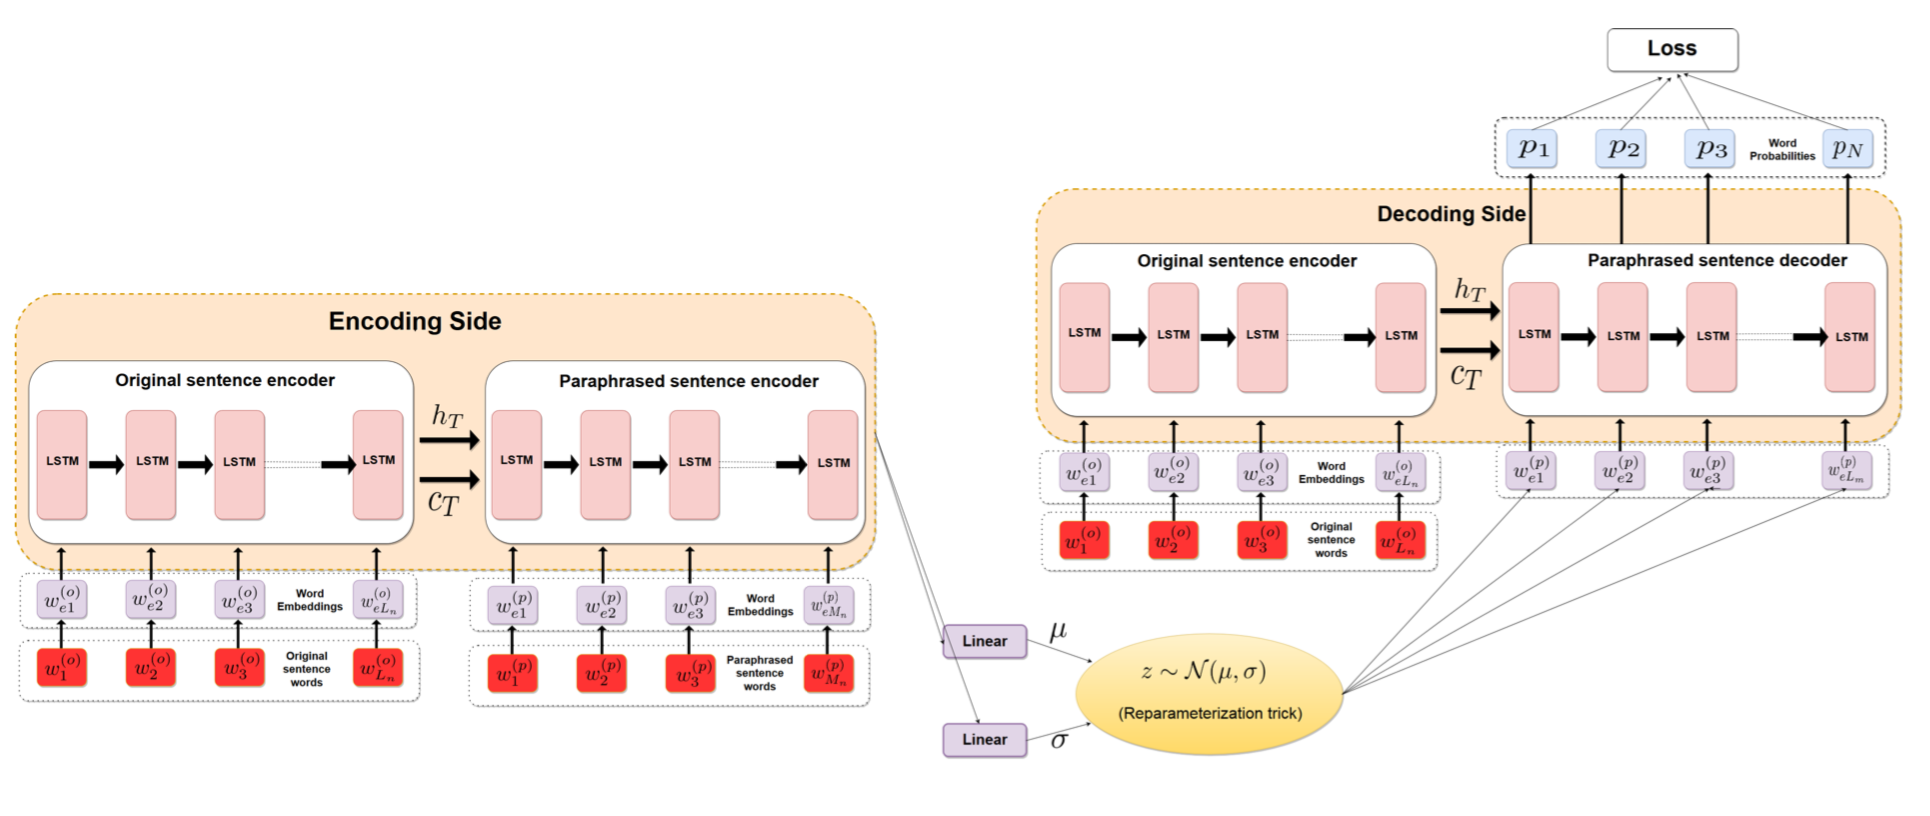
\includegraphics[width=12cm, height=6cm]{A_Deep_Framework_for_Text_Paraphrasing.png}
\end{frame}

\begin{frame}{Recent Existing Solutions}{Sequence-to-sequence Variational Autoencoder Model Cont.}
%-------------------------------------------------------
	\begin{block}{Encoder Side}
            \begin{itemize}
				\item {\tt Two of LSTMs encoders}
                \item {\tt the first one converts the original sentence into vector representation \textbf{(Skip-thought)}}
                \item {\tt The second one encoded the paraphrased sentence as well}
                \item {\tt The two vector representations are fed into Feedforward Network to estimate the VAE's mean and variance}
			\end{itemize}
	\end{block}
    
    \begin{block}{Sampling}
            \begin{itemize}
				\item {\tt Use the estimated parameters to produce a sample from a distribution that is parameterized by the estimated mean and variance}
			\end{itemize}
	\end{block}
\end{frame}

\begin{frame}{Recent Existing Solutions}{Sequence-to-sequence Variational Autoencoder Model Cont.}

\begin{block}{Decoder Side}
            \begin{itemize}
				\item {\tt The VAE’s output side uses an LSTM decoder which takes as input the latent representation and the vector representation of the original sentence}
                \item {\tt Both latent representation and the original sentence representation are used to reconstruct the paraphrased sentence}
                \item {\tt In the testing phase, we only concern on the decoder side and ignore the encoding side. We take the decoding side and feed it with the input sentence that we want to get its paraphrased version}
			\end{itemize}
	\end{block}
\end{frame}

\begin{frame}{Recent Existing Solutions}{Sequence-to-sequence Variational Autoencoder Model Cont.}
Model Trivia
\begin{itemize}
	\item <1-> Simple \textbf{Kullback-leibler Divergence} cost function is used to estimate the model loss during the training phase
    \item <1-> Model is trained and evaluated on MSCOCO and Quora datasets
	\item <1-> Considered to be the current \textbf{state-of-the-art} model in Text Paraphrasing task
\end{itemize}
\end{frame}

%-------------------------------------------------------
\subsection{Stacked Residual LSTM Sequence-to-sequence Model}
\begin{frame}{Recent Existing Solutions}{Stacked Residual LSTM Sequence-to-sequence Model}
%-------------------------------------------------------
\centering
Neural Paraphrase Generation with Stacked Residual LSTM Networks \\
(Prakash et al. 2016)
\centering
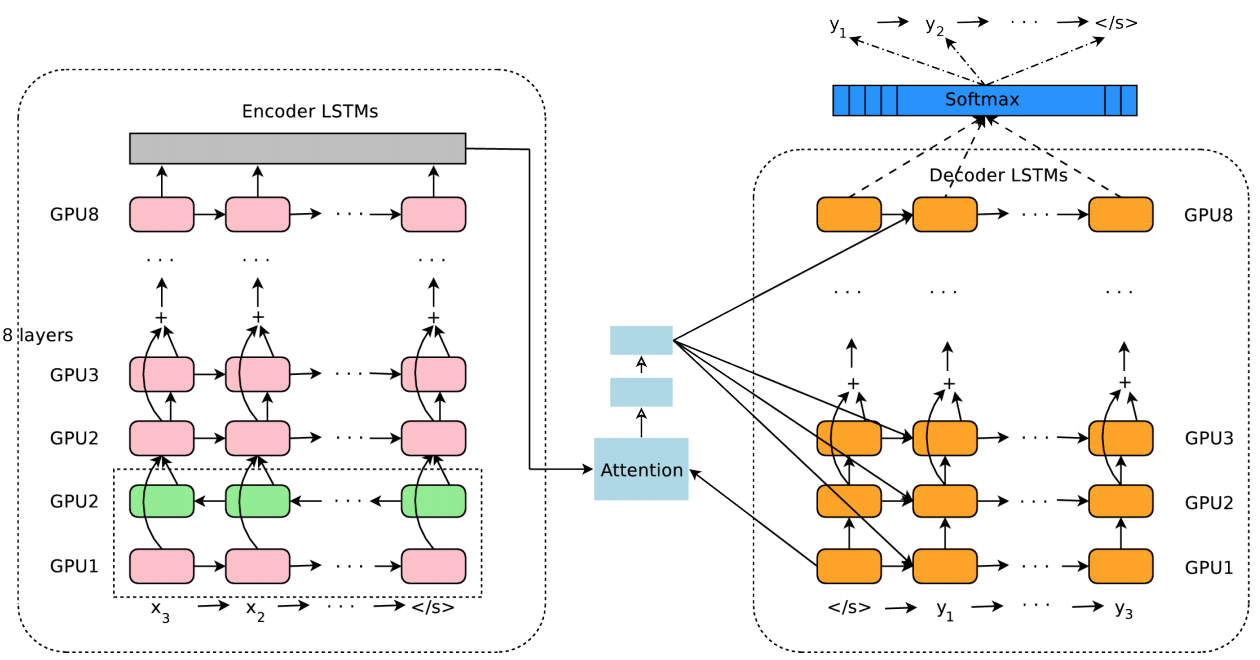
\includegraphics[width=11.5cm, height=6cm]{nmt.png}
\end{frame}

\begin{frame}{Recent Existing Solutions}{Stacked Residual LSTM Sequence-to-sequence Model Cont.}
%-------------------------------------------------------
\begin{block}{Encoder LSTMs}
            \begin{itemize}
				\item {\tt Residual Stacked LSTMs - They used only four layers}
                \item {\tt They used one-hot encoding for words representation}
                \item {\tt The input sentence is represented as a Skip-thought vector after applying the stacked LSTMs processes, which is fed into the decoder side}
			\end{itemize}
	\end{block}

\begin{block}{Decoder LSTMs}
            \begin{itemize}
				\item {\tt Residual Stacked LSTMs - They used only four layers}
                \item {\tt The input representation is fed to the decoder as the LSTMs initial state}
                \item {\tt Softmax layer to get the predicted word for each time step}
			\end{itemize}
	\end{block}
\end{frame}

\begin{frame}{Recent Existing Solutions}{Stacked Residual LSTM Sequence-to-sequence Model Cont.}
Model Trivia
\begin{itemize}
	\item <1-> The model is inspired from Google's Neural Machine Translation (NMT) Model. But they only used four stacked LSTMs instead of eight
    \item <1-> Beam Search algorithm was used to rank the best paraphrases candidates
    \item <1-> Model is trained and evaluated on MSCOCO and WikiAnswers and PPDB datasets
	\item <1-> Considered to be the first attempt in Text Paraphrasing task using Deep Learning model
\end{itemize}
\end{frame}


%-------------------------------------------------------
\subsection{Deep Reinforcement Learning Sequence-to-sequence Model}
\begin{frame}{Recent Existing Solutions}{Deep Reinforcement Learning Sequence-to-sequence Model}
%-------------------------------------------------------
\centering
Paraphrase Generation with Deep Reinforcement Learning \\
(Zichao et al. 2018)
\centering
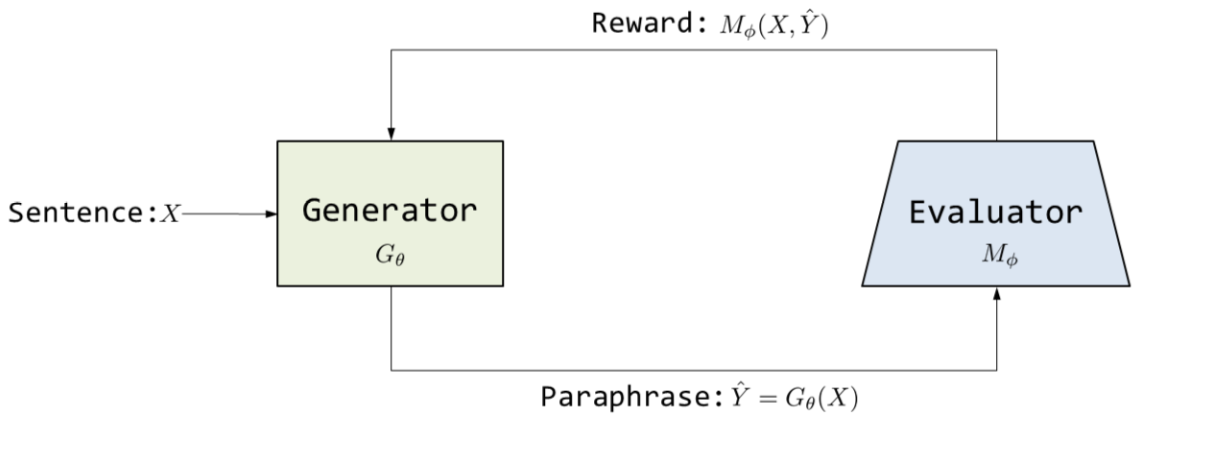
\includegraphics[width=12cm, height=6cm]{rl.png}
\end{frame}

\begin{frame}{Recent Existing Solutions}{Deep Reinforcement Learning Sequence-to-sequence Model}

\begin{block}{Generator}
	\begin{itemize}
    	\item <1-> A simple RNN sequence-to-sequence model
		\item <1-> The reinforcement part is that every paraphrased word is considered to be an action. The target is to maximize the profit and (the cross entropy in this situation) while generating the words
	\end{itemize}
\end{block}

\begin{block}{Evaluator}
	\begin{itemize}
    	\item <1-> Trained as a Supervised Learning model
		\item <1-> The model is trained using set of positive and negative examples (paraphrase pairs) as cross-entropy loss
        \item <1-> A well trained Evaluator forces the Generator to generate highly accurate paraphrased text
        \item <1-> This technique called Reinforced by Matching with Supervised Learning (RbM-SL)
	\end{itemize}
\end{block}
\end{frame}

\begin{frame}{Recent Existing Solutions}{Deep Reinforcement Learning Sequence-to-sequence Model Cont.}
Model Trivia
\begin{itemize}
	\item <1-> The model is considered to be the first attempt on using Reinforcement Learning in Text Paraphrasing problem
    \item <1-> Outperforms some of sequence-to-sequence models, such as \textbf{Vanilla Seq2Seq}, \textbf{Seq2Seq with Attention} and \textbf{Seq2Seq with Copy}
    \item <1-> Model is trained and evaluated on Quora dataset
\end{itemize}
\end{frame}

\section{Evaluation Metrics}
%-------------------------------------------------------
\subsection{BLEU, METEOR, WER Evaluation Metrics}
\begin{frame}{Evaluation Metrics}{BLEU, METEOR, WER}
%bilingual evaluation understudy
%-------------------------------------------------------
\begin{itemize}
\item <1-> Regularly, \textbf{BLEU}, \textbf{METEOR} and \textbf{WER} are the evaluation metrics that are used in any Text Generation task
\item <1-> In text paraphrasing, we will focues on \textbf{METEOR} metric as it matches between the input and output including word synonyms and hypernyms 
\end{itemize}
METEOR vs. BLEU
\begin{itemize}
\item <1-> \textbf{METEOR} word matches between input and output semantic equivalent
\item <1-> \textbf{METEOR} relies more on words ordering instead of \textbf{BLEU's} n-grams approach
\item <1-> \textbf{METEOR} has better correlation with human judgments, specially in short sentence level
\item <1-> \textbf{BLEU} works better in large sentences and paragraphs
\end{itemize}
\end{frame}

\section{References}
\textbf{References} \\
- A Deep Generative Framework for Paraphrase Generation - \href{https://arxiv.org/abs/1709.05074}{https://arxiv.org/abs/1709.05074} \\
- Neural Paraphrase Generation with Stacked Residual LSTM Networks - \href{https://arxiv.org/abs/1610.03098}{https://arxiv.org/abs/1610.03098} \\
- Paraphrase Generation with Deep Reinforcement Learning - \href{https://arxiv.org/abs/1711.00279}{https://arxiv.org/abs/1711.00279} \\
- Sequence to Sequence Learning with Neural Networks - 
 \href{https://arxiv.org/abs/1409.3215}{https://arxiv.org/abs/1409.3215} \\
- Generating Sentences from a Continuous Space - 
 \href{https://arxiv.org/abs/1511.06349}{https://arxiv.org/abs/1511.06349} \\
- Variational Recurrent Auto-Encoders
 - \href{https://arxiv.org/abs/1412.6581}{https://arxiv.org/abs/1412.6581} \\
- METEOR: An Automatic Metric for MT Evaluation with
Improved Correlation with Human Judgments - \href{https://www.cs.cmu.edu/~alavie/papers/BanerjeeLavie2005-final.pdf}{https://www.cs.cmu.edu/~alavie/papers/BanerjeeLavie2005-final.pdf} \\
- BLEU: A Method for Automatic Evaluation of Machine Translation \href{http://aclweb.org/anthology/P/P02/P02-1040.pdf}{http://aclweb.org/anthology/P/P02/P02-1040.pdf}

{\1
\begin{frame}[plain,noframenumbering]
  \finalpage{Thank you!}
\end{frame}}

\end{document}